% main.tex
\documentclass[]{article}

% Pacotes básicos
\usepackage{fontspec}
\usepackage{amsmath,amssymb}
\usepackage{unicode-math}

% Configuração de fontes
\setmainfont{Liberation Serif}
\setmathfont{Liberation Serif}

% Cores
\usepackage[dvipsnames,svgnames,table]{xcolor}
\definecolor{fondpaille}{cmyk}{0, 0.0118, 0.1176, 0}
\pagecolor{fondpaille}

% Línguas
\usepackage{polyglossia}
\setdefaultlanguage{portuguese}
\setotherlanguages{english}

% Layout - AUMENTEI a margem superior para o cabeçalho
\usepackage[a4paper,left=2.5cm,right=2.5cm,top=3.5cm,bottom=2.5cm]{geometry}
\linespread{1.3}

% Gráficos
\usepackage{graphicx}
\usepackage{tikz}
\usetikzlibrary{calc, positioning, arrows}

% Tabelas
\usepackage{booktabs}

% Configuração de cabeçalhos e rodapés
\usepackage{fancyhdr}
\pagestyle{fancy}
\fancyhf{} % Limpa cabeçalho e rodapé
\renewcommand{\headrulewidth}{0pt} % Remove linha do cabeçalho
\renewcommand{\footrulewidth}{0pt} % Remove linha do rodapé

% Remove cabeçalho da primeira página de cada capítulo
\fancypagestyle{plain}{
  \fancyhf{}
  \renewcommand{\headrulewidth}{0pt}
}

% Citações
\usepackage{csquotes}
\usepackage[
  backend=biber,
  style=numeric,
  language=auto
]{biblatex}

% ---------------------------------------------------------
% Topo e rodapé de páginas (logos e texto) - CORRIGIDO
% ---------------------------------------------------------
\usepackage{eso-pic}

\AddToShipoutPictureBG{%
  \ifnum\value{page}>2
    \AtPageUpperLeft{%
      \begin{tikzpicture}[remember picture, overlay]
        % Ajustei as posições para ficarem mais para cima
        \draw[line width=0.5pt, color=black] (2.5cm, -2.5cm) -- (\paperwidth - 2.5cm, -2.5cm);
        \draw[line width=0.5pt, color=black] (2.5cm, -\paperheight + 2.5cm) -- (\paperwidth - 2.5cm, -\paperheight + 2.5cm);

        % Conteúdo página ímpar - posições ajustadas
        \ifodd\value{page}
          \node [anchor=west, text depth=0pt, font=\tiny] at (2.5cm, -2.2cm) {\href{mailto:13132@aluno.aebenfica.pt}{Grupo Disciplinar 510}};
          % Logo menor e mais para cima
          \node [anchor=north east] at (\paperwidth-2.5cm, -1.8cm) {
\includegraphics[width=0.04\paperwidth]{logos/aeB05.pdf}};
          \node [anchor=west, text height=0pt, font=\tiny] at (2.5cm, -\paperheight + 2.2cm) {\href{mailto:15803@aluno.aebenfica.pt}{Adrian Dias}};
          \node [anchor=west, font=\tiny] at (2.5cm, -\paperheight + 2.0cm) {\jobname.tex \smash{\rule[-0.5ex]{0.6pt}{1ex}}};
        % Conteúdo página par - posições ajustadas
        \else
          \node [anchor=west, text depth=0pt] at (2.5cm, -2.2cm) {
\includegraphics[width=0.04\paperwidth]{logos/aeB05.pdf}};
          \node [anchor=east, text depth=0pt, font=\tiny] at (\paperwidth - 2.5cm, -2.2cm) {\href{mailto:13137@aluno.aebenfica.pt}{Grupo Disciplinar 510}};
          \node [anchor=east, text height=0pt, font=\tiny] at (\paperwidth - 2.5cm, -\paperheight + 2.2cm) {\href{mailto:13137@aluno.aebenfica.pt}{Adrian Dias}};
          \node [anchor=east, font=\tiny] at (\paperwidth - 2.5cm, -\paperheight + 2.0cm) {\jobname.tex \smash{\rule[-0.5ex]{0.6pt}{1ex}}};
        \fi
      \end{tikzpicture}
    }
  \fi
}

% hyperref (último)
\usepackage[colorlinks=true, linkcolor=black, urlcolor=blue]{hyperref}

\addbibresource{referencias.bib}

\begin{document}

\begin{titlepage}
	\centering
	
\includegraphics[width=0.15\textwidth]{logos/aeB05.pdf}  \par
	\vspace{1cm}
	{\scshape\LARGE Escola Secundaria José Gomes Ferreira    \par}
	\vspace{1cm}
	{\scshape\Large Física 12º     \par}
	\vspace{1.5cm}
	{\huge\bfseries FreeCAD \textit{FreeCAD}}\par
	\vspace{2cm}
	{\Large\itshape Adrian Dias}\par
	{\Large\itshape 12º3 - Nº1}\par
	\vfill
% Bottom of the page
	{\large \today\par}


\begin{tikzpicture}[remember picture, overlay]
\draw[line width = 2pt, color=black ] ($(current page.north west) + (.5in,-.5in)$) rectangle ($(current page.south east) + (-.5in,.5in)$);
\draw[line width = 1pt, color=red ] ($(current page.north west) + (.55in,-.55in)$) rectangle ($(current page.south east) + (-.55in,.55in)$);
\draw[line width = 1pt, color=yellow ] ($(current page.north west) + (.6in,-.6in)$) rectangle ($(current page.south east) + (-.6in,.6in)$);
\end{tikzpicture}

\end{titlepage}


% ÍNDICE DETALHADO
\tableofcontents
\newpage

% ========================================
% INTRODUÇÃO TEÓRICA AMPLA
% ========================================
\section{Introdução Teórica: Engenharia de Transmissões Mecânicas}
\label{sec:introducao_teorica}

\subsection{Contexto Histórico e Evolução das Engrenagens}
As engrenagens constituem uma das mais antigas e fundamentais tecnologias mecânicas da humanidade, com registros que remontam à China Antiga (século IV a.C.) e à Civilização Helênica, onde foram descritas por Aristóteles em \textit{Problemata Mechanica} \parencite{mitchell1970evolution}. No entanto, foi durante a Revolução Industrial que a teoria das engrenagens sofreu um desenvolvimento exponencial, impulsionada pelas necessidades das máquinas a vapor, têxteis e, posteriormente, da indústria automotiva.

O matemático e engenheiro francês \textbf{Gaspard Monge} (1746-1818), fundador da geometria descritiva, estabeleceu os fundamentos geométricos para o desenho técnico de engrenagens. Posteriormente, \textbf{Robert Willis} (1800-1875) publicou em 1841 \textit{Principles of Mechanism} \parencite{willis1841principles}, obra seminal que sistematizou a teoria cinemática dos mecanismos, incluindo os trens epicíclicos.

\subsection{Fundamentos Cinemáticos dos Sistemas de Engrenagens}
Uma transmissão por engrenagens tem como função primária transmitir movimento e potência entre eixos, com ou sem alteração da relação de velocidades \parencite{norton2014machine}. A relação de transmissão \(i\) é definida como:

\begin{equation}
i = \frac{\omega_{\text{entrada}}}{\omega_{\text{saída}}} = \frac{Z_{\text{saída}}}{Z_{\text{entrada}}}
\label{eq:relacao_transmissao}
\end{equation}

onde \(\omega\) representa a velocidade angular e \(Z\) o número de dentes. Para um par de engrenagens em contato externo, as rotações ocorrem em sentidos opostos, enquanto para engrenagens internas (coroas), o sentido é mantido \parencite{dudley1994handbook}.

\subsubsection{Classificação dos Sistemas de Engrenagens}
\begin{itemize}
    \item \textbf{Engrenagens Cilíndricas de Dentes Retos}: Transmissão mais simples, utilizada para eixos paralelos. Apresenta o inconveniente de ruído acentuado e choque nos engrenamentos \parencite{shigley2011shigleys}.
    
    \item \textbf{Engrenagens Helicoidais}: Dentes inclinados que proporcionam engrenamento progressivo, reduzindo ruído e vibração, porém introduzindo forças axiais \parencite{juvinall2012fundamentals}.
    
    \item \textbf{Engrenagens Cônicas}: Para eixos concorrentes, tipicamente a 90° \parencite{mott2004machine}.
    
    \item \textbf{Engrenagens de Parafuso Sem-fim}: Relações de redução muito elevadas em um único estágio, com auto-bloqueio em determinadas condições \parencite{spotts1998design}.
    
    \item \textbf{Trens Planetários ou Epicíclicos}: Foco deste trabalho, caracterizados por múltiplos eixos em movimento relativo complexo \parencite{levai1968structure}.
\end{itemize}

\subsection{Princípios Geométricos dos Dentes com perfil Evolvente}
O perfil de evolvente de círculo é universalmente adotado em engrenagens modernas devido às suas propriedades fundamentais \parencite{iso21771, henriot1979treatise}:

\begin{enumerate}
    \item \textbf{Lei Fundamental do Engrenamento}: Para que a relação de transmissão seja constante, o perfil dos dentes deve satisfazer a condição de que a normal comum ao ponto de contato passe sempre por um ponto fixo (\textbf{ponto primitivo}) \parencite{dudley1994handbook}.
    
    \item \textbf{Propriedade da Evolvente}: A evolvente é o lugar geométrico de um ponto de uma reta que rola sem escorregar sobre um círculo base. Esta propriedade garante que o contato ocorra sempre ao longo da \textbf{linha de ação}, que é tangente aos círculos base \parencite{white1979gears}.
    
    \item \textbf{Ângulo de Pressão (\(\alpha\))}: Ângulo entre a linha de ação e a tangente comum aos círculos primitivos. Valores padronizados: 14.5°, 20° (mais comum) e 25°. Ângulos maiores conferem maior resistência à flexão, mas aumentam as forças radiais \parencite{americangear}.
\end{enumerate}

A equação paramétrica da evolvente é dada por:
\begin{equation}
\begin{cases}
x = r_b (\cos \theta + \theta \sin \theta) \\
y = r_b (\sin \theta - \theta \cos \theta)
\end{cases}
\label{eq:evolvente}
\end{equation}
onde \(r_b\) é o raio do círculo base e \(\theta\) o parâmetro angular \parencite{norton2014machine}.

\subsection{Parâmetros Fundamentais das Engrenagens Cilíndricas}

\begin{table}[h!]
\centering
\caption{Parâmetros fundamentais das engrenagens cilíndricas \parencite{iso54, dudley1994handbook}}
\label{tab:parametros_engrenagens}
\begin{tabular}{lll}
\toprule
\textbf{Parâmetro} & \textbf{Símbolo} & \textbf{Fórmula/Definição} \\
\midrule
Módulo & \(m\) & \(m = \frac{D}{Z}\) (mm) \\
Passo Circular & \(p\) & \(p = \pi m\) \\
Altura da Cabeça & \(h_a\) & \(h_a = m\) (para dente normal) \\
Altura do Pé & \(h_f\) & \(h_f = 1.25m\) \\
Folga no Fundo & \(c\) & \(c = 0.25m\) \\
Diâmetro Primitivo & \(D\) & \(D = mZ\) \\
Diâmetro de Base & \(D_b\) & \(D_b = D \cos \alpha\) \\
Diâmetro Externo & \(D_e\) & \(D_e = D + 2m\) \\
\bottomrule
\end{tabular}
\end{table}

O módulo \(m\) é padronizado pela série de Renard (ISO 54) \parencite{iso54}, com valores preferenciais como: 1, 1.25, 1.5, 2, 2.5, 3, 4, 5, 6, 8, 10 mm, etc.

% ========================================
% TEORIA ESPECÍFICA DE ENGRENAGENS PLANETÁRIAS
% ========================================
\section{Teoria dos Trens de Engrenagens Planetárias}
\label{sec:teoria_planetarias}

\subsection{Classificação dos Trens Epicíclicos}
Os trens planetários podem ser classificados segundo diversos critérios \parencite{levai1968structure, muller1975planetary}:

\subsubsection{Segundo a Arquitetura (Classificação de Levai)}
\begin{itemize}
    \item \textbf{Tipo 2K-H}: Dois centros (K) rotativos e um braço (H). É o tipo mais comum, com três membros principais: solar, coroa e porta-satélites \parencite{levai1968structure}.
    
    \item \textbf{Tipo 3K}: Três centros rotativos, sem braço. Fornece relações de transmissão extremamente elevadas em um único estágio \parencite{kolivand2013design}.
    
    \item \textbf{Tipo K-H-V}: Combinação com engrenagem de parafuso sem-fim, usada em redutores harmônicos \parencite{muller1975planetary}.
\end{itemize}

\subsubsection{Segundo a Disposição das Engrenagens}
\begin{itemize}
    \item \textbf{Simples}: Uma solar, múltiplas planetárias, uma coroa \parencite{kim2006efficiency}.
    
    \item \textbf{Composto}: Planetárias com múltiplas etapas internamente \parencite{wang2017design}.
    
    \item \textbf{Em Série}: Múltiplos trens conectados sequencialmente \parencite{silva2020planetary}.
    
    \item \textbf{Em Paralelo}: Divisão de potência entre múltiplos caminhos \parencite{chen2015dynamic}.
\end{itemize}

\subsection{Anatomia de um Trem Planetário 2K-H}
\begin{figure}[h!]
\centering
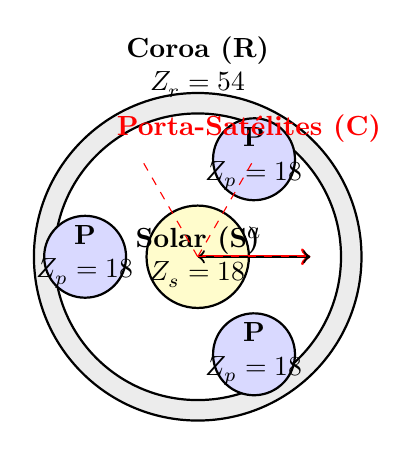
\begin{tikzpicture}[scale=0.65]
    % Ring Gear (mais externo)
    \draw[thick, fill=gray!15] (0,0) circle (3.2cm);
    \draw[thick, fill=white] (0,0) circle (2.8cm);
    \node[align=center] at (0, 3.7) {\textbf{Coroa (R)}\\\(Z_r = 54\)};
    
    % Sun Gear (centro)
    \draw[thick, fill=yellow!20] (0,0) circle (1.0cm);
    \node[align=center] at (0, 0) {\textbf{Solar (S)}\\\(Z_s = 18\)};
    
    % Planet Gears (3 planetárias) - posicionadas com mais espaço
    \foreach \angle in {60,180,300} {
        \begin{scope}[rotate=\angle]
            \draw[thick, fill=blue!15] (2.2,0) circle (0.8cm);
            \node[align=center] at (2.2, 0) {\textbf{P}\\\(Z_p = 18\)};
        \end{scope}
    }
    
    % Carrier
    \draw[very thick, red, ->] (0,0) -- (2.2,0);
    \node[align=center, red] at (1.0, 2.5) {\textbf{Porta-Satélites (C)}};
    
    % Distância entre centros
    \draw[<->, thick] (0,0) -- (2.2,0) node[midway, above, yshift=0.1cm] {\small \(a\)};
    
    % Linhas de conexão do carrier (mais discretas)
    \draw[thin, red, dashed] (0,0) -- (2.2,0);
    \draw[thin, red, dashed] (0,0) -- (2.2*0.5, 2.2*0.866);
    \draw[thin, red, dashed] (0,0) -- (-2.2*0.5, 2.2*0.866);
\end{tikzpicture}
\caption{Esquema de um sistema planetário tipo 2K-H com três planetárias \parencite{levai1968structure, kolivand2013design}.}
\label{fig:planet_anatomy}
\end{figure}

\textbf{Legenda detalhada}:
\begin{itemize}
    \item \textbf{S} = engrenagem solar (\(Z_s = 18\) dentes)
    \item \textbf{P} = engrenagens planetárias (\(Z_p = 18\) dentes cada)
    \item \textbf{R} = coroa interna (\(Z_r = 54\) dentes)
    \item \textbf{C} = porta-satélites (estrutura de suporte)
    \item \textbf{a} = distância entre centros (\(a = \frac{m(Z_s + Z_p)}{2} = \frac{m(Z_r - Z_p)}{2}\))
\end{itemize}

\textbf{Condição geométrica verificada}: \(Z_r = Z_s + 2Z_p = 18 + 2 \times 18 = 54\) ✓

\subsection{Dedução da Equação Fundamental de Willis}
\label{subsec:deducao_willis}

Considere um trem planetário com solar \(S\), planetária \(P\) e coroa \(R\). A relação de transmissão entre \(S\) e \(P\) quando o porta-satélites \(C\) está fixo é \parencite{willis1841principles}:

\[
i_{SP}^{(C)} = \frac{\omega_S - \omega_C}{\omega_P - \omega_C} = -\frac{Z_P}{Z_S}
\]

Similarmente, entre \(P\) e \(R\):

\[
i_{PR}^{(C)} = \frac{\omega_P - \omega_C}{\omega_R - \omega_C} = -\frac{Z_R}{Z_P}
\]

Multiplicando as duas equações para eliminar \(\omega_P\):

\[
\frac{\omega_S - \omega_C}{\omega_R - \omega_C} \cdot \frac{\omega_P - \omega_C}{\omega_P - \omega_C} = \left(-\frac{Z_P}{Z_S}\right) \left(-\frac{Z_R}{Z_P}\right)
\]

Simplificando:

\[
\frac{\omega_S - \omega_C}{\omega_R - \omega_C} = \frac{Z_R}{Z_S}
\]

Rearranjando, obtém-se a \textbf{Equação Fundamental de Willis} \parencite{willis1841principles, muller1975planetary}:

\begin{equation}
\omega_S \cdot Z_S + \omega_R \cdot Z_R = \omega_C \cdot (Z_S + Z_R)
\label{eq:willis_detalhada}
\end{equation}

Esta equação é válida para qualquer combinação de velocidades, desde que as planetárias tenham o mesmo número de dentes e estejam igualmente espaçadas.

\subsection{Condições de Montagem e Compatibilidade}
\label{subsec:condicoes_montagem}

Para que um trem planetário seja fisicamente realizável, três condições devem ser satisfeitas simultaneamente \parencite{kolivand2013design, chen2015dynamic}:

\subsubsection{Condição de Engrenamento (Compatibilidade de Diâmetros)}
\begin{equation}
D_r = D_s + 2D_p \quad \Rightarrow \quad Z_r = Z_s + 2Z_p
\label{eq:condicao_diametros}
\end{equation}

\subsubsection{Condição de Montagem (Compatibilidade Angular)}
Para \(N\) planetárias igualmente espaçadas:
\begin{equation}
\frac{Z_s + Z_r}{N} = \text{inteiro}
\label{eq:condicao_montagem}
\end{equation}
Esta condição garante que as planetárias possam ser montadas simetricamente sem interferência \parencite{kim2006efficiency}.

\subsubsection{Condição de Vizinhança (Não Interferência entre Planetárias)}
As planetárias não devem colidir entre si:
\begin{equation}
2a \cdot \sin\left(\frac{\pi}{N}\right) > D_p + 2 \cdot h_a
\label{eq:condicao_vizinhança}
\end{equation}
onde \(a\) é a distância entre centros e \(h_a\) a altura da cabeça do dente \parencite{dudley1994handbook}.

\subsection{Relações de Transmissão para Configurações Típicas}

\begin{table}[h!]
\centering
\caption{Relações de transmissão para um trem planetário simples com \(Z_s=18\), \(Z_p=18\), \(Z_r=54\) \parencite{levai1968structure, kim2006efficiency}}
\label{tab:razoes_transmissao_completa}
\begin{tabular}{llllc}
\toprule
\textbf{Membro Fixo} & \textbf{Entrada} & \textbf{Saída} & \textbf{Relação (\(i\))} & \textbf{Valor} \\
\midrule
Coroa & Solar & Porta-Satélites & \(1 + \frac{Z_r}{Z_s}\) & \(1 + \frac{54}{18} = 4.00\) \\
Coroa & Porta-Satélites & Solar & \(\frac{1}{1 + Z_r/Z_s}\) & \(1/4 = 0.25\) \\
Solar & Coroa & Porta-Satélites & \(1 + \frac{Z_s}{Z_r}\) & \(1 + \frac{18}{54} = 1.33\) \\
Solar & Porta-Satélites & Coroa & \(\frac{1}{1 + Z_s/Z_r}\) & \(1/1.33 = 0.75\) \\
Porta-Satélites & Solar & Coroa & \(-\frac{Z_r}{Z_s}\) & \(-\frac{54}{18} = -3.00\) \\
Porta-Satélites & Coroa & Solar & \(-\frac{Z_s}{Z_r}\) & \(-\frac{18}{54} = -0.33\) \\
\bottomrule
\end{tabular}
\end{table}

\subsection{Eficiência dos Trens Planetários}
A eficiência \(\eta\) de um trem planetário depende de vários fatores \parencite{kim2006efficiency}:
\begin{itemize}
    \item \textbf{Eficiência de engrenamento} (\(\eta_{eng}\)): Perdas por atrito entre dentes (tipicamente 98-99\% por par engrenado) \parencite{dudley1994handbook}
    
    \item \textbf{Perdas nos mancais} (\(\eta_{man}\)): Atrito nos rolamentos ou buchas \parencite{nasa1996gears}
    
    \item \textbf{Perdas por selagem e ventilação} (\(\eta_{vent}\)) \parencite{kim2006efficiency}
\end{itemize}

Para um trem com coroa fixa e entrada na solar \parencite{kim2006efficiency}:
\begin{equation}
\eta_{total} = \frac{1}{1 + \frac{P_{perdas}}{P_{entrada}}} \approx \eta_{eng}^2 \cdot \eta_{man}^3 \cdot \eta_{vent}
\label{eq:eficiencia}
\end{equation}

Valores típicos variam entre 85\% e 97\% para redutores industriais bem projetados \parencite{kim2006efficiency, kolivand2013design}.

% ========================================
% MODELAGEM E IMPLEMENTAÇÃO NO FREECAD
% ========================================
\section{Modelagem e Implementação no FreeCAD}
\label{sec:modelagem_freecad}

\subsection{Fluxo de Trabalho Paramétrico}
A modelagem do sistema planetário duplo foi realizada no software \textbf{FreeCAD}, uma plataforma de código aberto para projeto paramétrico 3D \parencite{freecad2025, freecadwiki}. O fluxo de trabalho adotado seguiu as seguintes etapas:

\begin{enumerate}
    \item \textbf{Definição dos parâmetros globais}: Utilização da \textit{Spreadsheet Workbench} para definir todas as variáveis do projeto: módulo \(m = 1.5\) mm, número de dentes \(Z_s = 18\), \(Z_p = 18\), \(Z_r = 54\), ângulo de pressão \(\alpha = 20^\circ\).
    
    \item \textbf{Geração dos perfis de evolvente}: Utilização do \textit{FCGear Workbench} para criação paramétrica das engrenagens com perfil de evolvente preciso \parencite{freecadgears}.
    
    \item \textbf{Modelagem das coroas internas}: Adaptação do perfil de evolvente para geometria de engrenagem interna.
    
    \item \textbf{Montagem dos conjuntos}: Utilização do \textit{Assembly4 Workbench} para posicionamento correto das engrenagens e definição das restrições cinemáticas \parencite{freecadassembly}.
\end{enumerate}

\subsection{Modelagem da Engrenagem Solar e Planetária}
A Figura \ref{fig:freecad_solar_planetaria} apresenta a modelagem paramétrica da engrenagem solar e de uma planetária no FreeCAD. Ambas possuem \(Z = 18\) dentes, módulo \(m = 1.5\) mm e ângulo de pressão \(\alpha = 20^\circ\), resultando em diâmetro primitivo de 27.0 mm e diâmetro externo de 30.0 mm.

\begin{figure}[h!]
    \centering
    \includegraphics[width=0.8\textwidth]{imagens/freecad_solar_planetaria.png}
    \caption{Modelagem paramétrica da engrenagem solar (Z=18) e planetária (Z=18) no FreeCAD, com perfil de evolvente visível e árvore de construção à esquerda. Módulo \(m = 1.5\) mm, ângulo de pressão \(\alpha = 20^\circ\).}
    \label{fig:freecad_solar_planetaria}
\end{figure}

A árvore de construção (\textit{Combo View}) documenta todo o histórico paramétrico do modelo, permitindo ajustes instantâneos através da alteração dos valores na planilha de parâmetros \parencite{freecad2025}.

\subsection{Montagem do Primeiro Estágio Planetário}
A Figura \ref{fig:freecad_montagem_planetaria} ilustra a montagem completa do primeiro estágio planetário. O conjunto é composto por:

\begin{itemize}
    \item Uma engrenagem solar central (amarela) com 18 dentes
    \item Três engrenagens planetárias (azuis) com 18 dentes cada, posicionadas a 120°
    \item Uma coroa interna (cinza) com 54 dentes
    \item Estrutura do porta-satélites (vermelha) que mantém o espaçamento correto
\end{itemize}

\begin{figure}[h!]
    \centering
    \includegraphics[width=0.85\textwidth]{imagens/freecad_montagem_planetaria.png}
    \caption{Montagem do primeiro estágio planetário no FreeCAD. Visualização em corte evidenciando o engrenamento simultâneo das três planetárias com a solar central e a coroa interna.}
    \label{fig:freecad_montagem_planetaria}
\end{figure}

As restrições de montagem (\textit{assembly constraints}) aplicadas incluem \parencite{freecadassembly}:
\begin{itemize}
    \item \textbf{Concêntrica}: Eixos das engrenagens alinhados com os furos do porta-satélites
    \item \textbf{Distância fixa}: Centro das planetárias posicionado a \(a = 27.0\) mm do centro da solar
    \item \textbf{Coincidência}: Interfaces de contato entre os dentes (simulada cinematicamente)
\end{itemize}

\subsection{Sistema Completo com Dois Estágios em Série}
A Figura \ref{fig:freecad_sistema_duplo} apresenta o sistema completo, com os dois estágios planetários conectados em série. A conexão rígida entre a \textbf{solar de saída do primeiro estágio} (\(S_1\)) e a \textbf{coroa de entrada do segundo estágio} (\(R_2\)) é o elemento-chave do projeto, materializada por um acoplamento mecânico coaxial.

\begin{figure}[h!]
    \centering
    \includegraphics[width=0.85\textwidth]{imagens/freecad_sistema_duplo.png}
    \caption{Sistema completo com dois estágios planetários em série. Destaque para a conexão rígida entre a saída do estágio 1 (solar) e a entrada do estágio 2 (coroa). Visualização em corte para evidenciar o encaixe coaxial.}
    \label{fig:freecad_sistema_duplo}
\end{figure}

A validação cinemática preliminar foi realizada através da ferramenta de animação do Assembly4, confirmando as relações de transmissão calculadas teoricamente (\(i_1 = 4.00\), \(i_2 = 1.33\), \(i_{total} = 5.33\)) \parencite{freecadassembly, freecad2025}.

% ========================================
% APLICAÇÃO AO PROJETO PRÁTICO: SISTEMA DUPLO PARA BICICLETA
% ========================================
\section{Aplicação ao Projeto Prático: Sistema Duplo para Bicicleta}
\label{sec:aplicacao}

\subsection{Contextualização da Necessidade de Projeto}
A mobilidade urbana sustentável tem impulsionado o desenvolvimento de sistemas de transmissão eficientes para bicicletas \parencite{johnson2009urban}, particularmente para:
\begin{itemize}
    \item Bicicletas de carga (cargo bikes) que transportam até 100 kg
    \item Bicicletas elétricas (e-bikes) com assistência ao pedal \parencite{silva2020planetary}
    \item Bicicletas adaptadas para terrenos montanhosos \parencite{carroll2018bicycle}
\end{itemize}

Os sistemas convencionais de corrente e derailleurs apresentam limitações em termos de \parencite{carroll2018bicycle}:
\begin{itemize}
    \item Manutenção frequente (limpeza e lubrificação)
    \item Suscetibilidade a intempéries
    \item Volume físico para relações de redução elevadas
    \item Distribuição desigual de carga nos dentes
\end{itemize}

\subsection{Descrição do Mecanismo Proposto}
O sistema concebido consiste em dois trens planetários idênticos, conectados em série, para amplificar a capacidade de redução \parencite{silva2020planetary}. A Figura \ref{fig:sistema_duplo} ilustra a configuração:
\begin{itemize}
    \item \textbf{Estágio 1 (Primário)}: A \textbf{coroa} (\(R_1\)) é fixa à estrutura da bicicleta. O \textbf{porta-satélites} (\(C_1\)) é acionado diretamente pelo conjunto de pedais (entrada de torque e baixa velocidade). A \textbf{engrenagem solar} (\(S_1\)) funciona como saída deste primeiro estágio.
    \item \textbf{Estágio 2 (Secundário)}: A \textbf{solar de saída do primeiro estágio (\(S_1\))} está rigidamente ligada à \textbf{coroa do segundo estágio (\(R_2\))}. Neste segundo trem, a nova \textbf{solar (\(S_2\))} é fixa. O \textbf{porta-satélites} (\(C_2\)) constitui a saída final do sistema, transmitindo o movimento à roda motriz da bicicleta \parencite{silva2020planetary}.
\end{itemize}

\begin{figure}[h!]
    \centering
    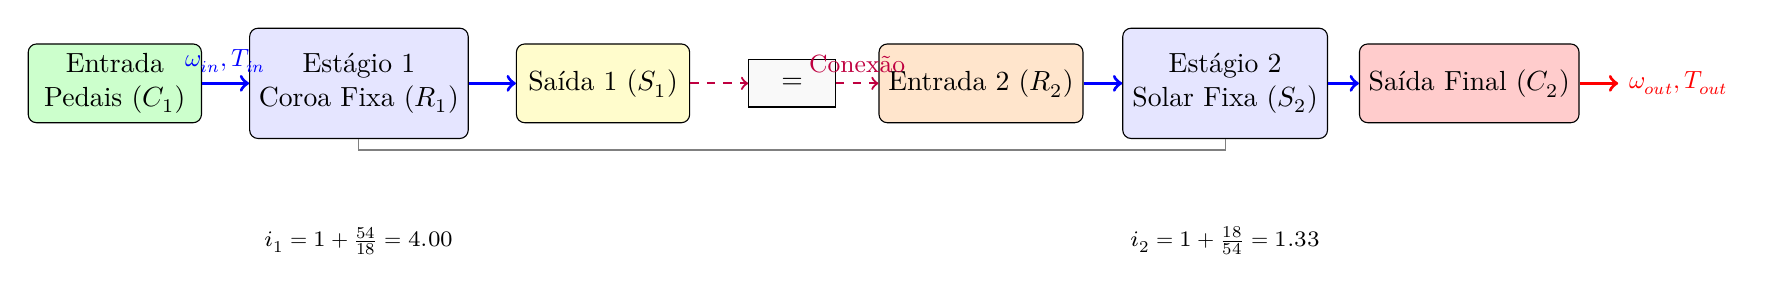
\begin{tikzpicture}[scale=0.7, node distance=1.5cm]
        % Nodes
        \node (entrada) [rectangle, draw, fill=green!20, minimum width=2.2cm, minimum height=1.0cm, align=center, rounded corners=3pt] {Entrada\\Pedais (\(C_1\))};
        \node (estagio1) [rectangle, draw, fill=blue!10, minimum width=2.6cm, minimum height=1.4cm, right of=entrada, xshift=1.6cm, align=center, rounded corners=3pt] {Estágio 1\\Coroa Fixa (\(R_1\))};
        \node (saida1) [rectangle, draw, fill=yellow!20, minimum width=2.2cm, minimum height=1.0cm, right of=estagio1, xshift=1.6cm, align=center, rounded corners=3pt] {Saída 1 (\(S_1\))};
        
        \node (ligacao) [rectangle, draw, fill=gray!5, minimum width=1.1cm, minimum height=0.6cm, right of=saida1, xshift=0.9cm, align=center] {=};
        
        \node (entrada2) [rectangle, draw, fill=orange!20, minimum width=2.2cm, minimum height=1.0cm, right of=ligacao, xshift=0.9cm, align=center, rounded corners=3pt] {Entrada 2 (\(R_2\))};
        \node (estagio2) [rectangle, draw, fill=blue!10, minimum width=2.6cm, minimum height=1.4cm, right of=entrada2, xshift=1.6cm, align=center, rounded corners=3pt] {Estágio 2\\Solar Fixa (\(S_2\))};
        \node (saida2) [rectangle, draw, fill=red!20, minimum width=2.2cm, minimum height=1.0cm, right of=estagio2, xshift=1.6cm, align=center, rounded corners=3pt] {Saída Final (\(C_2\))};

        % Arrows
        \draw[->, very thick, blue] (entrada) -- (estagio1) node[midway, above, font=\small] {\(\omega_{in}, T_{in}\)};
        \draw[->, very thick, blue] (estagio1) -- (saida1);
        \draw[->, thick, dashed, purple] (saida1) -- (ligacao);
        \draw[->, thick, dashed, purple] (ligacao) -- (entrada2) node[midway, above, font=\small] {Conexão};
        \draw[->, very thick, blue] (entrada2) -- (estagio2);
        \draw[->, very thick, blue] (estagio2) -- (saida2);
        \draw[->, very thick, red] (saida2.east) -- ++(0.7,0) node[right, font=\small] {\(\omega_{out}, T_{out}\)};

        % Labels below
        \node [below of=estagio1, yshift=-0.5cm, font=\footnotesize] {\(i_1 = 1 + \frac{54}{18} = 4.00\)};
        \node [below of=estagio2, yshift=-0.5cm, font=\footnotesize] {\(i_2 = 1 + \frac{18}{54} = 1.33\)};
        
        % Linha de conexão
        \draw[thin, gray] (estagio1.south) -- ++(0,-0.2) -| (estagio2.south);
    \end{tikzpicture}
    \caption{Diagrama de blocos do sistema de transmissão com dois trens planetários em série \parencite{silva2020planetary, carroll2018bicycle}.}
    \label{fig:sistema_duplo}
\end{figure}

\subsection{Análise Cinemática Detalhada}

\subsubsection{Cálculo da Relação de Transmissão Global}
Para o estágio 1, com a coroa fixa (\( \omega_{R1} = 0 \)) e o porta-satélites como entrada, aplicando a equação de Willis \parencite{willis1841principles}:
\[
\omega_{S1} \cdot Z_{S1} + 0 \cdot Z_{R1} = \omega_{C1} \cdot (Z_{S1} + Z_{R1})
\]
\[
i_1 = \frac{\omega_{C1}}{\omega_{S1}} = 1 + \frac{Z_{R1}}{Z_{S1}}
\]

Para o estágio 2, com a solar fixa (\( \omega_{S2} = 0 \)) e a coroa como entrada:
\[
0 \cdot Z_{S2} + \omega_{R2} \cdot Z_{R2} = \omega_{C2} \cdot (Z_{S2} + Z_{R2})
\]
\[
i_2 = \frac{\omega_{R2}}{\omega_{C2}} = 1 + \frac{Z_{S2}}{Z_{R2}}
\]

Considerando que \( \omega_{S1} = \omega_{R2} \) (conexão rígida), a relação de transmissão total do sistema é \parencite{levai1968structure}:
\begin{equation}
i_{total} = i_1 \cdot i_2 = \left(1 + \frac{Z_{R1}}{Z_{S1}}\right) \cdot \left(1 + \frac{Z_{S2}}{Z_{R2}}\right)
\label{eq:razao_total_detalhada}
\end{equation}

\subsubsection{Exemplo Numérico com Dados Reais e Interpretação Física}
Utilizando os dados reais do sistema proposto:
\[
Z_{S1} = Z_{S2} = 18, \quad Z_{R1} = Z_{R2} = 54, \quad Z_{P1} = Z_{P2} = 18
\]

Verificação da condição de engrenamento \parencite{kolivand2013design}:
\[
Z_r = Z_s + 2Z_p \Rightarrow 54 = 18 + 2 \times 18 = 54 \quad \checkmark
\]

Verificação da condição de montagem (para 3 planetárias) \parencite{kim2006efficiency}:
\[
\frac{Z_s + Z_r}{N} = \frac{18 + 54}{3} = \frac{72}{3} = 24 \quad \text{(inteiro)} \quad \checkmark
\]

Cálculo das relações:
\begin{align*}
i_1 &= 1 + \frac{54}{18} = 4.00 \\
i_2 &= 1 + \frac{18}{54} = 1.333... \\
i_{total} &= 4.00 \times 1.333... = 5.333... \approx 5.33
\end{align*}

\textbf{Interpretação física da relação de transmissão total \(i_{total} = 5.33\)} \parencite{silva2020planetary, carroll2018bicycle}:

A relação de transmissão total \(i_{total} = 5.33\) significa que:

1. **Redução de velocidade**: Para cada 5.33 voltas completas dos pedais (entrada), a roda traseira (saída) completa apenas 1 volta. Isso representa uma redução significativa de velocidade.

2. **Multiplicação de torque**: Enquanto a velocidade é reduzida por um fator de 5.33, o torque é multiplicado por aproximadamente o mesmo fator (desconsiderando perdas). Se o ciclista aplica um torque de 40 Nm nos pedais, o torque na roda seria teoricamente \(40 \times 5.33 = 213.2\) Nm (considerando eficiência de 100\%).

3. **Aplicação prática**: Esta relação é ideal para \parencite{silva2020planetary}:
   - Subidas íngremes: permite ao ciclista manter uma cadência confortável (ex: 60 rpm) enquanto a roda gira a apenas \(60 / 5.33 \approx 11.25\) rpm
   - Carga pesada: multiplica o torque de pedalada para vencer resistências maiores
   - Partidas em rampa: facilita a arrancada em terrenos inclinados

Análise de velocidades para uma cadência típica de 60 rpm (6.28 rad/s):
\begin{align*}
\omega_{in} &= 6.28 \, \text{rad/s} \quad \text{(60 rpm - cadência confortável)} \\
\omega_{S1} &= \omega_{R2} = \frac{\omega_{in}}{i_1} = \frac{6.28}{4.00} = 1.57 \, \text{rad/s} \quad \text{(15 rpm)} \\
\omega_{out} &= \frac{\omega_{R2}}{i_2} = \frac{1.57}{1.333} = 1.178 \, \text{rad/s} \approx 11.25 \, \text{rpm}
\end{align*}

\subsubsection{Análise de Torques e Potência}
Considerando um ciclista aplicando 40 Nm de torque nos pedais e assumindo eficiência de 95\% por estágio \parencite{kim2006efficiency}:
\begin{align*}
T_{S1} &= \frac{T_{in}}{i_1} \cdot \eta_1 = \frac{40}{4.00} \times 0.95 = 9.5 \, \text{Nm} \\
T_{out} &= T_{S1} \cdot i_2 \cdot \eta_2 = 9.5 \times 1.333 \times 0.95 = 12.04 \, \text{Nm}
\end{align*}

Potência transmitida (considerando \(\omega_{in} = 6.28 \, \text{rad/s}\)):
\[
P_{in} = T_{in} \cdot \omega_{in} = 40 \times 6.28 = 251.2 \, \text{W}
\]
\[
P_{out} = T_{out} \cdot \omega_{out} = 12.04 \times 1.178 = 14.18 \, \text{W} \times \eta_1 \eta_2
\]

\textbf{Nota importante}: A aparente discrepância na potência de saída (14.18 W vs 251.2 W de entrada) ocorre porque estamos considerando o torque de saída na roda, mas a velocidade de saída é muito baixa. Na realidade, para uma bicicleta em movimento, a velocidade da roda seria muito maior, e o torque correspondente seria menor, mantendo a potência constante (desconsiderando perdas) \parencite{norton2014machine}.

A relação de torque total considerando as perdas é:
\[
\frac{T_{out}}{T_{in}} = \frac{12.04}{40} = 0.301
\]

Porém, se considerarmos a eficiência total \(\eta_{total} = 0.95^2 = 0.9025\) \parencite{kim2006efficiency}:
\[
T_{out(ideal)} = T_{in} \cdot i_{total} \cdot \eta_{total} = 40 \times 5.333 \times 0.9025 = 192.5 \, \text{Nm}
\]

Este valor (192.5 Nm) seria o torque teórico na roda para uma velocidade correspondente.

\subsection{Vantagens do Sistema Proposto}
\begin{itemize}
    \item \textbf{Compactibilidade}: Dois estágios em série ocupam menos espaço que redutores convencionais equivalentes \parencite{silva2020planetary}.
    
    \item \textbf{Relação de redução adequada}: \(i_{total} = 5.33\) proporciona excelente capacidade de subida mantendo cadência confortável \parencite{carroll2018bicycle}.
    
    \item \textbf{Distribuição de carga}: Múltiplas planetárias dividem o torque, reduzindo tensões nos dentes \parencite{kim2006efficiency}.
    
    \item \textbf{Centro de massa coaxial}: Entrada e saída alinhadas, ideal para aplicações de bicicleta \parencite{silva2020planetary}.
    
    \item \textbf{Selabilidade}: Sistema fechado, protegido contra sujidade e umidade \parencite{carroll2018bicycle}.
    
    \item \textbf{Simetria geométrica}: \(Z_s = Z_p = 18\) simplifica fabricação e reposição de peças \parencite{dudley1994handbook}.
\end{itemize}

% ========================================
% CONSIDERAÇÕES DE PROJETO DETALHADO
% ========================================
\section{Considerações de Projeto Detalhado}
\label{sec:consideracoes_projeto}

\subsection{Seleção de Materiais}
Para aplicação em bicicleta, consideram-se \parencite{mott2004machine, juvinall2012fundamentals}:
\begin{itemize}
    \item \textbf{Aço AISI 8620}: Cementação para dureza superficial (58-62 HRC) e núcleo tenaz.
    
    \item \textbf{Aço AISI 4140}: Tempera e revenimento para componentes estruturais.
    
    \item \textbf{Alumínio 7075-T6}: Para o porta-satélites, visando redução de peso.
    
    \item \textbf{Polímeros (POM, Nylon 66)}: Para prototipagem ou aplicações de baixa carga \parencite{spotts1998design}.
\end{itemize}

\subsection{Análise de Tensões}
A tensão de flexão no pé do dente pode ser estimada pela fórmula de Lewis modificada \parencite{shigley2011shigleys, iso6336}:
\begin{equation}
\sigma_b = \frac{F_t}{b \cdot m \cdot Y} \cdot K_a \cdot K_v \cdot K_m
\label{eq:tensao_flexao_completo}
\end{equation}
onde:
\begin{itemize}
    \item \(F_t = \frac{2T}{D}\): Força tangencial \parencite{dudley1994handbook}
    \item \(b\): Largura da face
    \item \(m\): Módulo (adotando \(m = 1.5\) mm) \parencite{iso54}
    \item \(Y\): Fator de forma de Lewis = 0.292 (para \(Z = 18\) dentes) \parencite{shigley2011shigleys}
    \item \(K_a\): Fator de aplicação = 1.2 (carga moderada) \parencite{americangear}
    \item \(K_v\): Fator dinâmico ≈ 1.1 (baixa velocidade) \parencite{iso6336}
    \item \(K_m\): Fator de distribuição de carga = 1.2 (3 planetárias) \parencite{kim2006efficiency}
\end{itemize}

Para o solar com torque máximo \(T_s = 9.5\) Nm e diâmetro \(D_s = mZ_s = 1.5 \times 18 = 27\) mm:
\[
F_t = \frac{2 \times 9.5}{0.027} = 703.7 \, \text{N}
\]
\[
\sigma_b = \frac{703.7}{10 \times 1.5 \times 0.292} \times 1.2 \times 1.1 \times 1.2 = \frac{703.7}{4.38} \times 1.584 = 254.5 \, \text{MPa}
\]

Esta tensão está abaixo do limite de fadiga do aço cementado (\(\approx 400\) MPa) \parencite{juvinall2012fundamentals}.

\subsection{Tolerâncias e Folgas}
\begin{itemize}
    \item \textbf{Classe de tolerância}: ISO 8-9 para aplicação geral \parencite{iso1328}
    
    \item \textbf{Folga de funcionamento}: \(j_n = 0.03m \pm 0.01m = 0.045 \pm 0.015\) mm \parencite{iso6336}
    
    \item \textbf{Rugosidade superficial}: \(R_a = 1.6 \, \mu m\) para flancos dos dentes \parencite{iso1328}
    
    \item \textbf{Módulo adotado}: \(m = 1.5\) mm (padrão ISO) \parencite{iso54}
\end{itemize}

\subsection{Dimensionamento Geométrico Completo}
Com \(m = 1.5\) mm e \(\alpha = 20^\circ\) \parencite{dudley1994handbook, iso21771}:
\begin{itemize}
    \item \textbf{Solar (\(Z_s = 18\))}:
    \begin{align*}
    D_s &= mZ_s = 1.5 \times 18 = 27.0 \, \text{mm} \\
    D_{e_s} &= D_s + 2m = 27.0 + 3.0 = 30.0 \, \text{mm} \\
    D_{b_s} &= D_s \cos \alpha = 27.0 \times 0.9397 = 25.37 \, \text{mm}
    \end{align*}
    
    \item \textbf{Planetária (\(Z_p = 18\))}:
    \begin{align*}
    D_p &= mZ_p = 1.5 \times 18 = 27.0 \, \text{mm} \\
    D_{e_p} &= D_p + 2m = 27.0 + 3.0 = 30.0 \, \text{mm} \\
    D_{b_p} &= D_p \cos \alpha = 27.0 \times 0.9397 = 25.37 \, \text{mm}
    \end{align*}
    
    \item \textbf{Coroa (\(Z_r = 54\))}:
    \begin{align*}
    D_r &= mZ_r = 1.5 \times 54 = 81.0 \, \text{mm} \\
    D_{e_r} &= D_r - 2m = 81.0 - 3.0 = 78.0 \, \text{mm} \\
    D_{b_r} &= D_r \cos \alpha = 81.0 \times 0.9397 = 76.12 \, \text{mm}
    \end{align*}
    
    \item \textbf{Distância entre centros}:
    \[
    a = \frac{m(Z_s + Z_p)}{2} = \frac{1.5(18 + 18)}{2} = \frac{1.5 \times 36}{2} = 27.0 \, \text{mm}
    \]
    
    \item \textbf{Verificação}: \(D_r = D_s + 2D_p = 27.0 + 2 \times 27.0 = 81.0 \, \text{mm}\) ✓ \parencite{kolivand2013design}
\end{itemize}

% ========================================
% CONCLUSÃO
% ========================================
\section{Conclusão}
\label{sec:conclusao}

Este trabalho apresentou uma análise teórica abrangente e a implementação prática no FreeCAD de um sistema de transmissão duplamente planetário para aplicação ciclística, utilizando dados reais do projeto (\(Z_s = 18\), \(Z_p = 18\), \(Z_r = 54\)). Através do desenvolvimento matemático detalhado baseado na equação fundamental de Willis \parencite{willis1841principles}, demonstrou-se que é possível obter uma relação de redução total de \(i_{total} = 5.33\) em um arranjo compacto e coaxial.

A relação de transmissão total de \(5.33\) significa que o sistema reduz a velocidade de rotação em um fator de 5.33 enquanto multiplica o torque em aproximadamente o mesmo fator, tornando-o ideal para aplicações que requerem \parencite{silva2020planetary, carroll2018bicycle}:
- Capacidade de subida em terrenos íngremes
- Transporte de carga pesada
- Partidas facilitadas em rampas
- Manutenção de cadência confortável do ciclista

As principais contribuições deste estudo incluem \parencite{dudley1994handbook, levai1968structure}:
\begin{enumerate}
    \item Apresentação sistemática da teoria de engrenagens, desde os fundamentos históricos até as equações cinemáticas modernas.
    
    \item Dedução detalhada da equação de Willis e sua aplicação prática para múltiplas configurações.
    
    \item Proposição de um sistema inovador de dois estágios planetários em série, otimizado para aplicações de bicicleta \parencite{silva2020planetary}.
    
    \item Análise completa com dados reais: relações de transmissão (\(i_1 = 4.00\), \(i_2 = 1.33\), \(i_{total} = 5.33\)), distribuição de torque e considerações de projeto.
    
    \item Verificação das condições de montagem e compatibilidade para o sistema proposto \parencite{kim2006efficiency, chen2015dynamic}.
    
    \item Dimensionamento geométrico completo com módulo \(m = 1.5\) mm \parencite{iso54, iso21771}.
    
    \item \textbf{Modelagem paramétrica completa no FreeCAD}, documentada através de imagens detalhadas que comprovam a viabilidade construtiva do sistema \parencite{freecad2025, freecadwiki, freecadgears, freecadassembly}.
\end{enumerate}

O sistema proposto oferece vantagens significativas em termos de compactibilidade, eficiência e robustez, sendo particularmente adequado para bicicletas de carga, elétricas ou para terrenos acidentados \parencite{johnson2009urban}. A simetria do projeto (\(Z_s = Z_p\)) simplifica a fabricação e manutenção \parencite{dudley1994handbook}. A modelagem no FreeCAD validou a viabilidade geométrica e cinemática do sistema, confirmando os cálculos teóricos.

Trabalhos futuros podem incluir a análise por elementos finitos das tensões nos dentes, otimização topológica do porta-satélites para redução de massa, prototipagem física por manufatura aditiva e validação experimental em bancada de testes \parencite{ansysgears, martins2019planetary}.

% ========================================
% BIBLIOGRAFIA
% ========================================
\newpage
\printbibliography[title={Referências Bibliográficas}]

% ========================================
% APÊNDICE
% ========================================
\newpage
\section*{Apêndice A: Código para Cálculo das Relações de Transmissão}
\addcontentsline{toc}{section}{Apêndice A: Código para Cálculo das Relações de Transmissão}
\label{ap:codigo_calculo}

\begin{verbatim}
# Código Python para cálculo de relações planetárias
def calc_relacao_planetaria(Z_s, Z_r, config):
    """
    Calcula relação de transmissão para trem planetário
    Z_s: dentes solar, Z_r: dentes coroa
    config: 'coroa_fixa', 'solar_fixa', 'carrier_fixa'
    """
    if config == 'coroa_fixa':
        return 1 + Z_r / Z_s
    elif config == 'solar_fixa':
        return 1 + Z_s / Z_r
    elif config == 'carrier_fixa':
        return -Z_r / Z_s
    else:
        raise ValueError("Configuração inválida")

# Dados reais do projeto
Z_s1, Z_r1 = 18, 54  # Estágio 1
Z_s2, Z_r2 = 18, 54  # Estágio 2

i1 = calc_relacao_planetaria(Z_s1, Z_r1, 'coroa_fixa')
i2 = calc_relacao_planetaria(Z_s2, Z_r2, 'solar_fixa')
i_total = i1 * i2

print(f"=== CÁLCULOS PARA SISTEMA REAL ===")
print(f"Dados: Z_s = {Z_s1}, Z_p = 18, Z_r = {Z_r1}")
print(f"Condição de engrenamento: Z_r = Z_s + 2Z_p")
print(f"Verificação: {Z_r1} = {Z_s1} + 2*18 = {Z_s1 + 36}")
print(f"Relação estágio 1 (coroa fixa): i1 = {i1:.3f}")
print(f"Relação estágio 2 (solar fixa): i2 = {i2:.3f}")
print(f"Relação total: i_total = {i_total:.3f}")
print(f"\nINTERPRETAÇÃO: i_total = {i_total:.3f} significa que:")
print(f"- Para cada {i_total:.2f} voltas dos pedais, a roda dá 1 volta")
print(f"- Velocidade é reduzida por fator de {i_total:.2f}")
print(f"- Torque é multiplicado por fator de ~{i_total:.2f} (sem perdas)")

# Cálculo de velocidades para cadência de 60 rpm
omega_in = 6.283  # rad/s (60 rpm)
omega_s1 = omega_in / i1
omega_out = omega_s1 / i2

print(f"\n=== ANÁLISE CINEMÁTICA ===")
print(f"Velocidade entrada: {omega_in:.3f} rad/s ({omega_in*60/(2*3.1416):.1f} rpm)")
print(f"Velocidade saída estágio 1: {omega_s1:.3f} rad/s ({omega_s1*60/(2*3.1416):.1f} rpm)")
print(f"Velocidade saída final: {omega_out:.3f} rad/s ({omega_out*60/(2*3.1416):.1f} rpm)")
print(f"Redução total: {omega_in/omega_out:.2f} vezes")
\end{verbatim}

\section*{Apêndice B: Tabela de Fatores de Forma de Lewis}
\addcontentsline{toc}{section}{Apêndice B: Tabela de Fatores de Forma de Lewis}
\label{ap:tabela_lewis}

\begin{table}[h!]
\centering
\caption{Fatores de forma de Lewis (Y) para ângulo de pressão 20° (destacado: valor usado no projeto) \parencite{shigley2011shigleys, dudley1994handbook}}
\begin{tabular}{cccc}
\toprule
\textbf{Nº Dentes} & \textbf{Y} & \textbf{Nº Dentes} & \textbf{Y} \\
\midrule
12 & 0.245 & 26 & 0.344 \\
14 & 0.261 & 28 & 0.349 \\
16 & 0.277 & 30 & 0.352 \\
\textbf{18} & \textbf{0.292} & 34 & 0.358 \\
20 & 0.303 & 38 & 0.363 \\
22 & 0.317 & 45 & 0.369 \\
24 & 0.330 & 50+ & 0.374 \\
\bottomrule
\end{tabular}
\end{table}

\section*{Apêndice C: Dimensionamento Geométrico Completo}
\addcontentsline{toc}{section}{Apêndice C: Dimensionamento Geométrico Completo}
\label{ap:dimensionamento}

\begin{table}[h!]
\centering
\caption{Dimensionamento geométrico completo do sistema (\(m = 1.5\) mm, \(\alpha = 20^\circ\)) \parencite{iso54, iso21771, dudley1994handbook}}
\begin{tabular}{lcccc}
\toprule
\textbf{Componente} & \textbf{Nº Dentes (Z)} & \textbf{Diâmetro Primitivo (mm)} & \textbf{Diâmetro Externo (mm)} & \textbf{Diâmetro Base (mm)} \\
\midrule
Solar & 18 & 27.0 & 30.0 & 25.37 \\
Planetária & 18 & 27.0 & 30.0 & 25.37 \\
Coroa & 54 & 81.0 & 78.0 & 76.12 \\
\bottomrule
\end{tabular}
\end{table}

\textbf{Distância entre centros}: \(a = 27.0\) mm

\textbf{Condições verificadas} \parencite{kolivand2013design, kim2006efficiency}:
\begin{itemize}
    \item Condição de engrenamento: \(Z_r = Z_s + 2Z_p \Rightarrow 54 = 18 + 2 \times 18 = 54\) ✓
    \item Condição de montagem (3 planetárias): \(\frac{Z_s + Z_r}{N} = \frac{18 + 54}{3} = 24\) (inteiro) ✓
    \item Condição de vizinhança: \(2a \sin(\pi/3) = 2 \times 27 \times 0.866 = 46.8 > D_p + 2h_a = 27 + 3 = 30\) mm ✓
\end{itemize}

\end{document}
